\documentclass[fleqn]{article}
\usepackage[nodisplayskipstretch]{setspace}
\usepackage{amsmath, nccmath, bm}
\usepackage{amssymb}
\usepackage{enumitem}
\usepackage{etoolbox}
\usepackage{graphicx}
\usepackage{float}
\usepackage{changepage}
\usepackage{environ,capt-of}

\let\oldfigure\figure% Store original figure float environment
\let\endoldfigure\endfigure
\RenewEnviron{figure}[1][H]{% Update figure environment
  %\par\vspace{\intextsep}% Assume in-text placement, so insert appropriate vertical spacing
  \noindent
  % \patchcmd{<cmd>}{<search>}{<replace>}{<success>}{<failure>}
  \patchcmd{\BODY}{\caption}{\captionof{figure}}{}{}% Replace \caption with \captionof{figure} inside \BODY
  % Set "figure"
  \begin{minipage}{\linewidth}
    \BODY
  \end{minipage}
  %\par\vspace{\intextsep}% Assume in-text placement, so insert appropriate vertical spacing
}

\newcommand{\zerodisplayskip}{
	\setlength{\abovedisplayskip}{0pt}%
	\setlength{\belowdisplayskip}{0pt}%
	\setlength{\abovedisplayshortskip}{0pt}%
	\setlength{\belowdisplayshortskip}{0pt}%
	\setlength{\mathindent}{0pt}}
	
\title{Homework 4}
\author{Owen Sowatzke}
\date{March 29, 2024}

\begin{document}

	\offinterlineskip
	\setlength{\lineskip}{12pt}
	\zerodisplayskip
	\maketitle
	
	\begin{enumerate}
		\item Show that if the activation function of the hidden layer is linear, a three layer network is equivalent to a two layer one.
		
		\begin{figure}[H]
			\centerline{\fbox{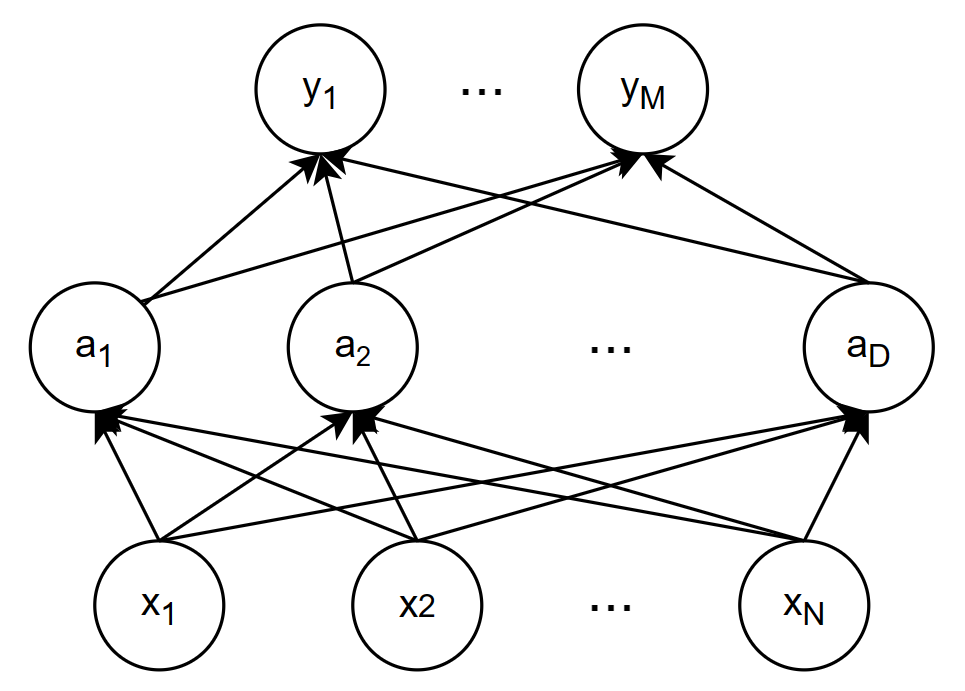
\includegraphics[width=0.4\textwidth]{neural_network_3_layer.png}}}
			\caption{3-Layer Neural Network}
			\label{neural_network_3_layer}
		\end{figure}
	
	\end{enumerate}
\end{document}